\chapter{Analysis of Interface Roughness based on Diffuse Scattering} \label{ch_diff}
With the detailed analysis based on the combination of several complementary experimental methods and the \gls{mcmc} evaluation performed in chapter~\ref{ch_spec}, reconstructions and confidence intervals for the model parameters for all sample systems could be obtained. It was found that roughness and intermixing or interdiffusion are of high relevance to explain the diminished reflectivity observed. Most prominently, the interface morphology in the Mo/Si/C sample system from Sec.~\ref{ch_spec:sec_mo_si_c} had a large effect on the reflectivity behavior in both the polished and unpolished case. We attributed the observations to the occurrence of a crystallization process in the molybdenum layer, which affects the interface morphology. Similarly, in case of the Cr/Sc mirror system presented in Sec.~\ref{ch_spec:sec_CrSc}, intermixing or interdiffusion and roughness were attributed to cause the large gap between theoretical reflectivity predictions and actual values measured in the experiments.

So far, no distinction was made between interdiffusion or intermixing and roughness at the surface or interfaces. As discussed in detail in Sec.~\ref{ch_spec:sec_CrSc_results}, this distinction based on the employed methods is in fact not possible due to the lack of sensitivity of the experiments conducted there not even for the combination of all methods. Due to the comparatively large beam footprint on the sample in comparison to interfacial roughness on the nanoscale, any specular reflection measurement, and even the measurement of fluorescence radiation generated by a standing wave field, is only sensitive to the average of the interfacial profile and can thus not be distinguished from horizontally homogeneous intermixing. Effectively, both cases can be described with a gradual profile in the optical constants at the interfaces. Consequently, all methods applied so far rely on a horizontally homogeneous medium model, which was reconstructed. The correlation of the roughness parameter $\sigma$ and the intermixing parameter $\eta$ in Fig.~\ref{ch_spec:fig_CrSc_eta_rho_correlation} of Sec.~\ref{ch_spec:sec_CrSc_results} nicely demonstrate that assessment.

Within this chapter, we investigate the diffuse scattering contribution measured from all samples studied in chapter~\ref{ch_spec}. While none of the experiments conducted there could yield a distinction criterion, diffuse scattering can only be observed from rough surfaces or interfaces, while intermixing and interdiffusion do not cause any off-specular intensity contribution. The analysis of the diffuse scattering, here in particular scattering in the \gls{euv} spectral range, therefore serve as a natural tool to implement the distinction of intermixing or interdiffusion on the one hand and roughness on the other. In addition, the distribution of the scattered intensity contains information on the morphology of roughness which is of particular interest to understand the effect on the reflectivity as observed in Sec.~\ref{ch_spec:sec_mo_si_c} and Sec.~\ref{ch_spec:sec_CrSc}. First, in Sec.~\ref{ch_diff:sec_PTB17}, we continue the analysis of the Mo/B$_4$C/Si/C sample based on the reconstruction found in Sec.~\ref{ch_spec:sec_reconstruction_PTB17} and demonstrate in detail the effects observed in case of diffuse \gls{euv} scattering from multilayer systems with an analysis based on the theory introduced in Sec.~\ref{ch_theo:sec_diffuse_scattering} of Ch.~\ref{ch_theo}. Second, in Sec.~\ref{ch_diff:sec_mo_si_c}, we analyze the effect of the crystallization presumed as cause for the diminished reflectivity observed for some of the samples in the two sets of Mo/Si/C systems discussed in Sec.~\ref{ch_spec:sec_mo_si_c_results}. Furthermore, the effect of the polishing process in one of the sample sets on the interface morphology is addressed. Finally, in Sec.~\ref{ch_diff:sec_CrSc}, we resolve the parameter correlation of intermixing and roughness for the Cr/Sc sample and finalize the characterization made in Sec.~\ref{ch_spec:sec_CrSc_results}.


\section{Near-normal Incidence Diffuse Scattering} \label{ch_diff:sec_PTB17}
In the theoretical fundamentals on diffuse scattering in chapter~\ref{ch_theo}, we have elaborated on the characterization of the scatter intensity from a multilayer sample. The goal of the investigation of the diffuse scattering intensity is to relate the measurements to the interface morphology in the sample. In Sec.~\ref{ch_theo:sec_elastic_scattering}, the measured scattering intensity $I_\text{s}$ is described in terms of the differential scattering cross section $\big(\frac{d \sigma}{d \Omega}\big)$, which is given explicitly for the problem of interfacial and surface roughness in multilayer samples in Eq.~\eqref{ch_theo:eqn_full_dwba_expression}. As indicated there, the full theoretical description is based on the introduction of the reciprocal space as a unique set of coordinates for the scattering problem. This space is spanned by the coordinates $q_x$, $q_y$ and $q_z$. Those are the components of the momentum transfer due to the scattering process (cf.~Sec.~\ref{ch_theo:sec_diffuse_scattering}) and are related to the experimental parameters wavelength $\lambda$, as well as the angle of incidence $\alpha_i$ and the exit angle $\alpha_f$ of the scattering experiment. Based on the theory developed in Sec.~\ref{ch_theo:sec_diffuse_scattering}, a mapping of reciprocal space along the two coordinates $q_x$ and $q_z$ is required to obtain information on the samples interface morphology.

In order to discuss the diffuse scattering experiments and enable a theoretical analysis, we shall therefore first give some definitions of measurement geometry and how it is related to the reciprocal space coordinates. So far, any scattering measurement (excluding the \gls{xrf} experiment) of chapter~\ref{ch_spec} was conducted in the specular reflection geometry, where incidence and exit angle are equal,i.e.~at $q_x = q_y \equiv 0$. Diffusely scattered radiation caused by roughness, however, is scattered to off-specular angles. The experiments conducted here are exclusively done in a co-planar geometry since the roughness in the samples under investigation are assumed to be isotropic parallel to the surface and interfaces (cf.~Sec.~\ref{ch_theo:sec_diffuse_scattering}). Thus, any scattered radiation is only measured in the scattering plane defined by the incidence wave vector and the surface normal of the multilayer sample. Two different types of measurements need to be distinguished as they relate to different paths through reciprocal space, the \emph{detector scan} geometry and the \emph{rocking scan} geometry both indicated in Fig.~\ref{ch_diff:fig_scattering_geometry}.
\begin{figure}[htb]
    \def\svgwidth{0.6\textwidth}
    \import{svg/}{Streugeometrie_diffuse.pdf_tex}
    \caption{Co-planar measurement geometries. By keeping the opening angle $\Delta\Theta$ between incident and exit beam and the detector fixed, respectively, a rocking scan can be performed by changing the sample angle $\omega$. In a detector scan the sample angle $\omega$ is kept fixed and defines the angle of incidence while the detector is moved along $\Theta$.}
    \label{ch_diff:fig_scattering_geometry}
\end{figure}
The detector scan describes a movement of the detector inside the scattering plane recording radiation scattered to the exit angle $\alpha_f$, while keeping the incidence angle $\alpha_i$ (and the wavelength) constant and is indicated by the red shaded area in Fig.~\ref{ch_diff:fig_scattering_geometry}. The rocking scan refers to a rotation of the sample around the axis perpendicular to the scattering plane while keeping the detector position fixed with respect to the incident beam (indicated by the blue shaded are in Fig.~\ref{ch_diff:fig_scattering_geometry}). The angle between detector and the incident beam is referred to as $\Delta \Theta$, while the tilt angle of the sample is $\omega$. By changing $\omega$, the incidence angle $\alpha_i$ and the exit angle $\alpha_f$ are changed accordingly. In both cases this leads to incidence and exit angles, which are no longer equal and, thus, non-vanishing values for the $q_x$ vector component. The out-of-plane angle $\theta_f$ (cf.~Fig.~\ref{ch_theo:fig_scattering_process} in Ch.~\ref{ch_theo}) remains zero in those experiments and consequently $q_y \equiv 0$.

The corresponding paths through reciprocal space are different for these two cases. They are shown schematically in Fig.~\ref{ch_diff:fig_pathsInQ} for two exemplary experimental parameter sets of incidence angle $\alpha_i$ and opening angle $\Delta \Theta$, respectively,  as well as wavelength for the two scan types.
\begin{figure}[htb]
    \def\svgwidth{0.7\textwidth}
    \import{svg/}{Qspace_paths.pdf_tex}
    \caption{Schematic positions in reciprocal space in dependence on the measurement geometry. The dashed path represents a rocking scan with the angle $\omega$. The solid line shows the movement in $q$-space when changing the detector angle $\Theta$ at a fixed angle of incidence. By tuning the wavelength at each angular position, the $q_z$-direction becomes accessible as indicated by the dotted arrows.}
    \label{ch_diff:fig_pathsInQ} 
\end{figure}
Clearly, for a mapping of the two-dimensional space spanned by $q_x$ and $q_z$ it does not suffice to perform only angular scans. In addition,wavelength scans ($\lambda$-scan) have to be performed at each angular position. By changing the wavelength and the angle in the same measurement, both degrees of freedom ($q_x$ and $q_z$) in reciprocal space become accessible.

Based on the theory in Sec.~\ref{ch_theo:sec_diffuse_scattering}, the \gls{psd} describing the statistical properties of the samples roughness contributes to the scattering intensity being only dependent on the variable $q_x$ (generally dependent on $q_\parallel = \sqrt{q_x^2+q_y^2}$, which reduces to $q_\parallel \equiv q_x$ in co-planar geometry), i.e.~the momentum transfer within the interface planes. There, we have derived an expression for the \gls{psd}, which describes an average value across all interfaces of the multilayer. The reason for that is that due to the high quality of the multilayer system, correlation of roughness perpendicular to the stack was assumed, which we shall verify here based on the diffuse scattering experiments. Furthermore, it should be noted that individual \gls{psd}s are theoretically possible but pose an ill-defined model for the experiment conducted here. In all measurements taken here, all interfaces contribute to the diffuse scattering intensity. The experiment thus delivers a statistical average across all interfaces, which makes a distinction of individual interfaces impossible.

Based on the \gls{psd} as derived in Eq.~\eqref{ch_theo:eqn_psd} with the dependence only on $q_x$, we should expect to be able to extract its values from the measured data as cuts along the $q_x$ axis anywhere in a measured reciprocal space map. However, it was observed by others in grazing incidence diffuse x-ray scattering experiments, that vertical correlation of roughness causes an additional intensity modulation of the scattering in reciprocal space along the $q_z$ direction, the so-called \emph{Bragg sheets} \cite{jiang_nonspecular_1992, holy_nonspecular_1994, salditt_kinetic_1994, holy_interface_1995}. As the interfaces have periodic distances along the surface normal of the sample, roughness correlation poses an additional Bragg condition enhancing the diffuse scattering where fulfilled. Since the periodicity of the interfaces is the multilayer periodicity, those Bragg sheets are expected to appear, where the first and higher order Bragg condition of the multilayer is fulfilled, i.e.~where $q_z=2 m \tilde{n} D$. Here, $m$ is the integer number of the Bragg order, $D$ is the multilayer period thickness and $\tilde{n}$ the average index of refraction. Those sheets of increased intensity vary in thickness along $q_z$ depending on the strength of the correlation of roughness along the vertical direction in the sample. The higher the correlation, the thinner is the Bragg sheet in $q_z$ direction. In the theoretical treatment of the diffuse scattering, this vertical roughness correlation enters as a replication factor in Eq.~\eqref{ch_theo:eqn_reduced_structure_factor} and can be explicitly derived by modeling the layer growth based on the Langevin equation Eq.~\eqref{ch_theo:eqn_langevin} and is given by Eq.~\eqref{ch_theo:eqn_replication_factor}. Due to the strong enhanced intensity in those Bragg sheets, the \gls{psd} is preferably extracted as a vertical cut along $q_x$ at the $q_z$ position of the sheet \cite{siffalovic_characterization_2009}. Consequently, in the following we shall focus on the mapping of reciprocal space in the vicinity of the first Bragg resonance to observe the expected Bragg-sheet intensity distribution and analyze the interface morphology.

In contrast to most of the studies cited above, reciprocal space maps of multilayer diffuse scattering so far have been conducted in a grazing incidence geometry using X-rays. The major disadvantage of this technique is that curved samples are not accessible in that way, since no grazing incidence measurement can be conducted. Here, we study the diffuse scattering using \gls{euv} radiation impinging near-normal incidence. Thereby, this disadvantage is overcome. However, as explained above, using near-normal incidence radiation requires a tuneablility of the wavelength to gain access to the $q_z$ direction in reciprocal space, whereas grazing incidence studies reveal the Bragg sheets in the out-of-plane direction at fixed photon energies, e.g.~\textcite{siffalovic_characterization_2009}.

%Following this method, we recorded two-dimensional reciprocal space maps of the vicinity of the first Bragg resonance. The reciprocal space coordinates in terms of the experimental parameters are given by 
%\begin{align}
% 	q_x &= \frac{2 \pi}{\lambda} \big(\sin(\Theta) - \sin(\alpha_i)\big) \text{,}\\
% 	q_z &= \frac{2\pi}{\lambda} \big(\cos(\Theta) + \cos(\alpha_i)\big) \text{,} 
% \end{align}
% where $\lambda$ is the wavelength of the incoming light, $\Theta$ is the exit angle with respect to the surface normal (detector angle) and $\alpha_i$ is the angle of incidence with respect to the surface normal.





\subsection{Mapping Reciprocal Space for the Mo/B$_4$C/Si/C Sample}
In this section we investigate the \gls{euv} diffuse scattering from the Mo/B$_4$C/Si/C sample discussed in Sec.~\ref{ch_spec:sec_PTB17} of Ch.~\ref{ch_spec} as an example for the analysis of near-normal scatter intensity from multilayer samples. In Sec.~\ref{ch_spec:sec_reconstruction_PTB17}, a reconstruction based on the measurement of \gls{euv} reflectivity curves was found and the values listed in table~\ref{ch_spec:tbl_mo_b4c_si_c_multilayer_mcmc_results} as \emph{PSO result} serve as the model parameters for the analysis conducted here.

We have conducted diffuse scattering measurements in three different geometries at the \gls{sx700} beamline at \gls{bessy}. A GaAsP photo diode with an active area of $\mm{4.5} \times \mm{4.5}$ at a distance to the sample of $\mm{250}$ was used as a detector for the diffusely scattered radiation. The reciprocal space maps were recorded for the two rocking scan geometries with at an opening angle of $\Delta \Theta = 13.5^\circ$ and of $\Delta \Theta = 30^\circ$ (corresponding to an angle of incidence of $\alpha_i = 6.75^\circ$ and $\alpha_i = 15.0^\circ$, respectively, in specular geometry), respectively, and for the detector scan geometry with the angle of incidence fixed at $\alpha_i = 6.75^\circ$. The first Bragg peak for this multilayer sample, due to its design, is in the wavelength range between \nm{12.4} and \nm{14.0}. At each angular position of the aforementioned angular scan geometries, a wavelength scan was conducted in this range using a step size of $\Delta \lambda = \nm{0.01}$. The angular ranges for the rocking scan with opening angle $\Delta \Theta = \SI{13.5}{\degree}$ correspond to angles of incidence from $\alpha_i = \SI{-18.0}{\degree}$ to $\alpha_i = \SI{31.5}{\degree}$ in steps of $\Delta\alpha_i = \SI{0.5}{\degree}$. In terms of the rocking angle $\omega$ this range corresponds to values from $\omega = \SI{-24.75}{\degree}$ to $\omega = \SI{24.75}{\degree}$, where $\omega = \SI{0.0}{\degree}$ corresponds to the specular reflection geometry ($\alpha_i = \alpha_f$). For the second rocking scan geometry with $\Delta \Theta = \SI{30.0}{\degree}$, the angle of incidence was varied from $\alpha_i = \SI{-3.0}{\degree}$ to $\alpha_i = \SI{27.5}{\degree}$ (corresponding to $\omega = \SI{-18.0}{\degree}$ to $\omega = \SI{12.5}{\degree}$) in steps of $\SI{0.5}{\degree}$. Finally, the detector scan was performed at an angle of incidence of $\alpha_i = \SI{6.75}{\degree}$ moving the detector from $\alpha_f = \SI{-3.75}{\degree}$ to $\alpha_f = \SI{46.75}{\degree}$ (corresponding to detector angles from $\Delta \Theta = \SI{3.0}{\degree}$ to $\Delta \Theta = \SI{40.0}{\degree}$) also in steps of $\SI{0.5}{\degree}$. From the experimental values, the respective reciprocal space coordinates were calculated and the corresponding maps are shown together in direct comparison in Fig.~\ref{ch_diff:fig_PTB17_detector_and_rocking_maps}.
\begin{figure*}[htbp]
        \includegraphics[width=
        \textwidth]{img/PTB17_diffuse_scattering_multiple_geometries} \caption{Measured intensity map of a detector scan of the Mo/B$_4$C/Si/C multilayer mirror at an angle of incidence $\alpha_i = 6.75^\circ$ (a) and measured intensity maps of the identical sample obtained through rocking scans at an opening angle between detector and incident beam of $\Delta \Theta = 13.5^\circ$ (b) and $\Delta \Theta = 30^\circ$ (c). The area close to the specular axis was excluded from this dataset due to its strong intensity compared to the diffuse scattering shown here. The access to the negative $q_x$-axis in (a) is limited due clipping of the incoming beam with the detector.} \label{ch_diff:fig_PTB17_detector_and_rocking_maps}
\end{figure*}

The reciprocal space maps in Fig.~\ref{fig:comparison} for the rocking scan (b) at an opening angle of $\Delta \Theta = 13.5^\circ$ and the rocking scan (c) at an opening angle of $\Delta \Theta = 30^\circ$ and for the detector scan with the angle of incidence $\alpha_i = 6.75^\circ$ clearly show different symmetries rather than the expected Bragg sheet. We observe a strong enhancement in the off-specular scattering around $q_x\approx0.1$ nm$^{-1}$ (cf.~Fig.~\ref{fig:comparison}(a) and Fig.~\ref{fig:comparison}(c)), which is not replicated on the negative $q_x$-axis in case of (a). The rocking scans \ref{fig:comparison}(b) and \ref{fig:comparison}(c) are symmetric with respect to the specular axis at $q_x=0$, however, no enhanced scattering appears in (b). The latter map shows a triangular-shaped intensity distribution for both the positive and 
negative $q_x$ range. A minimum in width with respect to the $q_z$ direction can be observed here around $q_x \approx \pm 0.2$ nm$^{-1}$. The triangular shape also appears for the 
positive $q_x$ range 
of the detector scan in Fig.~\ref{fig:comparison}(a), where the minimum in width coincides with the intensity maximum. These observations are in clear contrast to the expectation of an appearance of identical Bragg sheets, independent of the measurement geometry. Clearly, the measurement of diffuse scattering at \gls{euv} wavelengths and near-normal incidence differs from the observations made for grazing incidence experiments using X-rays (cf.~\textcite{salditt_kinetic_1994} or \textcite{jiang_nonspecular_1992}).

The measurement geometry dependence of the reciprocal space maps indicates that the intensity distributions cannot be the result of multilayer roughness properties alone, i.e.~the power spectral density. Scattering intensities caused by roughness occur at identical positions in reciprocal space for any measurement geometry. In fact, the additional modulations of the scatter intensity are caused by the direction from which the radiation impinges on the multilayer structure itself, rather than the roughness properties. Starting from the theoretical description, the contributions observed here are therefore clearly a direct result of the field amplitudes at the interfaces as described in the theory chapter~\ref{ch_theo:sec_diffuse_scattering} entering the full expression for the differential scattering cross section in Eq.~\eqref{ch_theo:eqn_full_dwba_expression}. To better understand the effects involved here, we shall analyze the intensity curves for all three measurement geometries based on a horizontal cut along $q_x$ at the position of $q_z=\SI{0.93}{\nano\meter^{-1}}$, which corresponds to the momentum transfer at the multilayer resonance and thus the maximum of the Bragg sheet and contain the \gls{psd} analogous to \textcite{siffalovic_characterization_2009}. The intensity curves are shown in direct comparison in Fig.~\ref{ch_diff:fig_PTB17_qx_cuts_different_geometries}
\begin{figure}[htbp]
	\includegraphics{img/PTB17_diffuse_BraggSheet_DetectorAndRocking} \caption{Averaged diffuse scattering intensity along $q_x$ in the interval  $q_z=(0.930 \pm 0.003$) nm$^{-1}$ corresponding to the resonance of the multilayer. The data shown are two rocking scan and one detector scan geometries (see text for details).} \label{ch_diff:fig_PTB17_qx_cuts_different_geometries}
\end{figure}
The strong off-specular enhancement of scattering intensity is clearly visible here for the detector scan geometry and the rocking scan with opening angle of $\Delta\Theta = \SI{30.0}{\degree}$. In case of the second rocking scan with $\Delta\Theta = \SI{13.5}{\degree}$, only a small shoulder can be observed at $q_x \approx \pm \SI{0.2}{\nano\meter^{-1}}$.


\subsection{Kiessig-like Peaks and Resonant Effects}
    \begin{align}
        {\underset{\text{DWBA}}{\Big(\frac{d \sigma}{d \Omega}\Big)}} = &\textcolor{fit_color}{\Bigg[\frac{A \pi^2}{\lambda^4}\sum \limits_{j=1}^{N}\sum \limits_{i=1}^{N} (n_j^2 - n_{j+1}^2)^* (n_i^2 - n_{i+1}^2)\Big( (T^{(1)}_j + R^{(1)}_j)^* (T^{(2)}_j + R^{(2)}_j)^*} \nonumber \\ &\textcolor{fit_color}{\qquad\times(T^{(1)}_i + R^{(1)}_i) (T^{(2)}_i + R^{(2)}_i) \Big) \exp\Big(-i q_x \tan \beta (z_i-z_j)\Big) c_\perp^{i j}\Bigg]}\,\, \textcolor{data_color}{C(q_x)} \text{.} \label{ch_diff:eqn_full_explicit_dwba_with_approximations}
    \end{align}
\begin{itemize}
\item Bragg-like peaks \cite{holy_nonspecular_1994}, \emph{Umweganregung} \cite{baumbach_influence_1994, baumbach_grazing-incidence_1995}
\end{itemize}
\begin{figure*}[htbp]
        \includegraphics[width=\textwidth]{img/kiessig_like_peaks_diffuse_map} \caption{Measured intensity map of a detector scan of a Mo/Si multilayer mirror at an angle of incidence $\alpha_i = 6.75^\circ$ (a) and  measured intensity maps of the identical sample obtained through rocking scans at an opening angle between detector and incident beam of $\Delta \Theta = 13.5^\circ$ (b) and $\Delta \Theta = 30^\circ$ (c). The area close to the specular axis was excluded from this dataset due to its strong intensity compared to the diffuse scattering shown here. The access to the negative $q_x$-axis in (a) is limited due clipping of the incoming beam with the detector.} \label{fig:comparison} 
\end{figure*}

\begin{figure*}[htb]
    %\def\svgwidth{\textwidth}
    \import{svg/}{Bragg_sheet_sheme.pdf_tex}
    \caption[Illustration of the four scattering processes of the DWBA.]{KLP}
    \label{ch_theo:fig_kiessig_like_peaks_scheme}
\end{figure*}

\label{sec:numerical_simulations} We have applied the theory above to the multilayer in our experiments. In order to obtain a model for the layer thicknesses in our multilayer, we measured the reflectivity of the sample in dependence on the wavelength. The recorded curve was fitted using the numerical calculation of the reflectivity curve based on the specular fields including the modified Fresnel coefficients in Eq.~\eqref{eqn:fresnel_r} and Eq.~\eqref{eqn:fresnel_t}. The resulting fit parameters were, then, further used to model the multilayer in the numerical simulations below. The fit of the reflectivity curve was later simultaneously optimized during the fit of the diffuse scattering in order to correct for the change in the mean roughness $\sigma$. The final thicknesses in the stack were fitted to $d_\text{Mo} = 2.0181$ nm, $d_\text{B$_4$C} = 1.3215$ nm, $d_\text{Si} = 3.0388$ nm and $d_\text{C} = 0.5858$ nm. The distorted-wave Born approximation was implemented in the \emph{Python} programming language using a highly parallel algorithm.

In order to determine the contribution of dynamic multiple reflections within the stack, we compared the semi-kinematic approximation in Eq.~\eqref{eqn:semi_kinematic_theory} with the dynamic calculations in Eq.~\eqref{eqn:multilayer_enhancement_factor}. For this comparison, we simulated a rocking scan at an opening angle of $\Delta \Theta = 30^\circ$ and compared the simulations with the measured data. The roughness properties for these simulations were determined following the procedure described below in Sec.~\ref{sec:determination_of_the_psd} including a discussion on the influence of the parameters, specifically $\xi_\perp(q_x)$, on these vertical line cuts.

A quantitative comparison of the dynamic contribution to the total scattering intensity in our measurements is shown in Fig.~\ref{fig:Comparison_full_semi} as a line cut along $q_z$ at $q_x=0.05$ nm$^{-1}$. The dynamic calculation yields excellent agreement with the measured data. The results show distinct differences with an increase up to 100\% of the scattered intensity close to the multilayer resonance at $q_z=0.93$ nm$^{-1}$ compared to the semi-kinematic calculation. Hence dynamic contributions are dominant in the vicinity of the Bragg resonance. 
\begin{figure}[htbp]
        \includegraphics{img/PTB17_diffuse_qz_kinematic_vs_dynamic_100nm} \caption{Scattering intensity along $q_z$ for $q_x=0.05$ nm$^{-1}$ for the dynamic and semi-kinematic calculations for a rocking scan at $\Delta\Theta=30^\circ$ in comparison to the measured data.} \label{fig:Comparison_full_semi} 
\end{figure}

To evaluate the contribution of multiple reflections due to the subsidiary maxima, Fig.~\ref{fig:kiessig_like_peak} shows the intensity distribution along $q_x$ at $q_z=0.93$ nm$^{-1}$.  These maxima are caused by interference of the reflections from the top surface of the multilayer stack and the substrate interface (Kiessig fringes) \cite{kiessig_interferenz_1931}.
\begin{figure*}[htbp]
        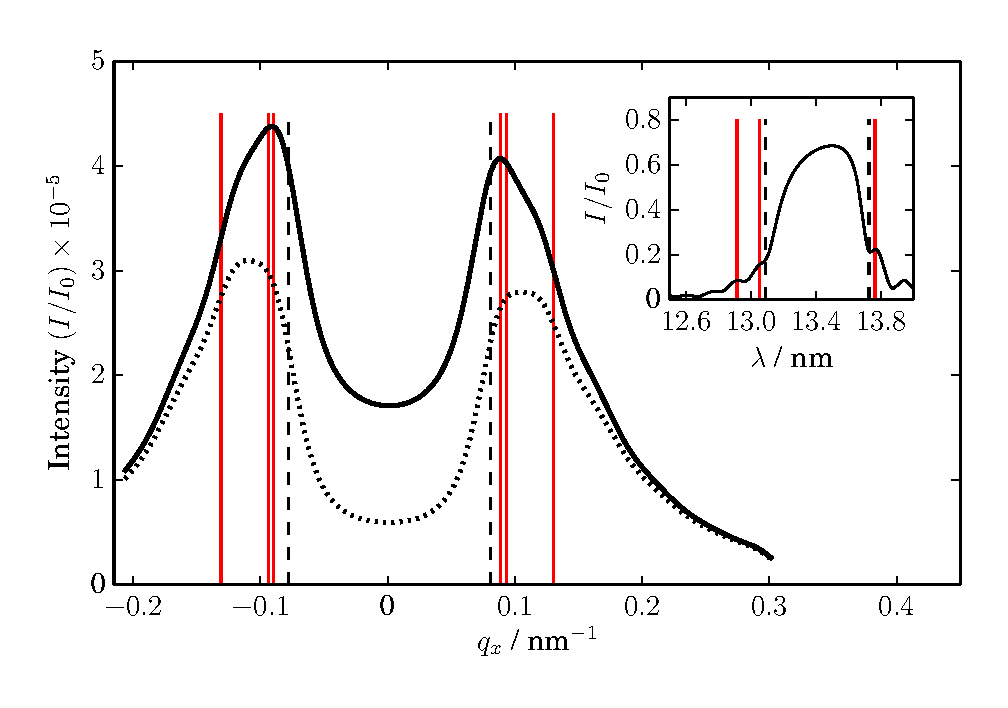
\includegraphics[width=\textwidth]{img/qx_kinematic_vs_dynamic}
        \caption{Scattering intensity distribution at $q_z=0.93$ nm$^{-1}$. The solid line shows the result of the dynamic calculation for a rocking scan with an opening angle of $\Delta\Theta=30^\circ$. The dashed line represents the calculation applying the semi-kinematic approximation, ignoring any multiple reflections within the multilayer. The dashed vertical lines are the limits of the main Bragg peak, while the red solid vertical lines show the position of dynamic contributions of the Kiessig fringes close to the main maximum. Each Kiessig fringe marked in the inset appears for the corresponding positive and negative $q_x$ value. The strong intensity at $q_x\approx0.1$ nm$^{-1}$ results from the overlap of the dynamic maxima of two different Kiessig fringes (see text).} \label{fig:kiessig_like_peak} 
\end{figure*}
The solid line corresponds to the dynamic theory, while the dotted line is the result of the semi-kinematic calculation. The dashed vertical lines indicate the limits of the main Bragg peak. These positions are defined through the first minimum on each side of the reflectivity peak (cf.~inset in Fig.~\ref{fig:kiessig_like_peak}). The vertical red lines show the position of multiple reflections due to Kiessig fringes close to the main resonance. Again, the corresponding positions in the specular reflectivity measurement are shown in the inset. Each of the marked fringes appears on the negative and positive $q_x$-axis in the main plot. This is caused by the incidence and exit angle, respectively, being at the resonance angle of the various Kiessig maxima in the reflectivity curve. Thus, a strong increase with respect to the semi-kinematic approximation is observed. The position of the dynamic contribution from the first 
Kiessig fringes on either side of the main resonance exhibits a pronounced maximum in the diffuse scattering. These fringes contribute most due to their high overall relative 
intensity compared with the fringes further away from the reflectivity maximum. In addition, the position in reciprocal space coincides with the first two Kiessig fringes marked on either side of the main maximum. This effect of dynamic maxima is similar to the observation of Bragg-like peaks in grazing incidence geometry \cite{kaganer_bragg_1995}, but it is caused by the subsidiary maxima instead. Consequently, we name this enhancement ``Kiessig-like peaks''. The contribution by the main Bragg resonance similar to the observations in Fig.~\ref{fig:Comparison_full_semi} amounts to approximately 100\% at $q_x=0$.


\subsection{Reconstruction of the PSD and the Multilayer Enhancement Factor}
\label{sec:multilayer_contribution}
The total contribution of the multilayer to the diffuse scattering, independent of lateral interface roughness properties, is described by the sum in the square brackets of Eq.~\eqref{eqn:multilayer_enhancement_factor} as a prefactor to the power spectral density $C(q_x)$. It describes the modulation of the scattering intensity due to the multilayer nature of the scattering structure, independent of the interface roughness. We thus consider it as a ``relative multilayer enhancement factor''. The result of the calculations based on the layer model of our multilayer sample is shown in Fig.~\ref{fig:MultilayerInfluence} for one detector and two rocking scan configurations. The vertical correlation length for this specific multilayer mirror is $\xi_\perp(q_x)=7.5/q_x^2$ nm$^{-1}$ as expected for a high-reflectance mirror, where $\xi_\perp$ 
exceeds the total thickness $D$ of the entire stack for $|q_x| < 0.12$ nm$^{-1}$. The method for the extraction of the vertical correlation length from the measured data is discussed in Sec.~\ref{sec:determination_of_the_psd}. The multilayer enhancement factor was normalized with respect to $q_x=0$, i.e. the calculated diffuse scattering contribution on the specular axis. 
\begin{figure}[htbp]
	\includegraphics{img/PTB17_multilayer_enhancement_factor} \caption{Enhancement factor due to the specific properties of multilayer reflectivity for three different measurement geometries. The simulations shown here were normalized with respect to the diffuse contribution to the specular reflectivity at $q_x=0$.} \label{fig:MultilayerInfluence} 
\end{figure}

The results clearly show that diffuse scattering from multilayers at near-normal incidence exhibit strong enhancement due to the intrinsically limited bandpass of reflectivity of multilayers. If both the incidence and exit angle is out of the Bragg resonance, the higher penetration depth of the multilayer causes an increase in the number of interfaces contributing to the diffuse scattering intensity. Thus higher total scattering is observed. The Kiessig fringes cause modulations in the enhancement factor increased by the purely dynamic processes described in Sec.~\ref{sec:dynamic_contributions}.

\begin{figure*}[htbp]
        \includegraphics[width=
        \textwidth]{img/PTB17_diffuse_simulation_vs_measurement} \caption{Measured (a) and simulated (b) reciprocal space maps for a rocking scan at an opening angle of $\Delta\Theta=30^\circ$ with the roughness parameters determined in Sec.~\ref{sec:determination_of_the_psd}.} \label{fig:comparisonWithTheory} 
\end{figure*}

\subsubsection{Reconstruction of the Power Spectral Density} \label{sec:determination_of_the_psd} In order to extract roughness properties from the off-specular measurements shown above, a correction for the influence of the multilayer as discussed in Sec.~\ref{sec:multilayer_contribution} is required. The scattering intensity after division by the multilayer enhancement factor represents the power spectral density of roughness. The measured PSDs are shown in Fig.~\ref{fig:PSDs_linear} for all three experiments. The excellent agreement with each other within the uncertainty margin confirms the validity and necessity of the dynamic theory to model the diffuse scattering from the multilayer. The reconstruction of the parameters of the power spectral density in Eq.~\eqref{eqn:psd} can be done by considering the overall intensity as well as the asymptotic behavior \cite{salditt_interfacial_1996} of the measured data in Fig.~\ref{fig:PSDs_linear}.

The numerical simulations show a strong sensitivity with respect to the mean roughness parameter $\sigma$ through the total portion of diffusely scattered light. As expected for a high-reflectance mirror, we obtained a small roughness value of $\sigma = 0.2$ nm.
\begin{figure}[htbp]
	\includegraphics{img/PTB17_PSD_for_all_geometries} \caption{Diffuse scattering intensity corrected for the multilayer enhancement factor considering a tilt angle of $\beta=-1^{\circ}$ according to Eq.~\eqref{eqn:tilt_correction}. The black solid line corresponds to a power spectral density with $\xi_\parallel=5.6$ nm, $H=1.0$, $\sigma=0.2$ nm and a vertical correlation length of $\xi_\perp(q_x)=7.5/q_x^2$ nm$^{-1}$.} \label{fig:PSDs_linear} 
\end{figure}

It follows from the definition of the PSD in Eq.~\eqref{eqn:psd} that the lateral correlation length $\xi_\parallel$ defines a cut-off for the spatial frequencies contributing to the off-specular scattering. We performed several simulations to compare the simulated intensity profile with the cut-off frequency observed in the measured data. A correlation length of $\xi_\parallel=5.6$ nm was obtained following this method. The fractal nature of the interfaces was analyzed by varying the Hurst parameter $H$. The asymptotic behavior of the power spectral density for $q_x>10^{-1}$~nm$^{-1}$ for the multilayer sample measured yields a Hurst factor of $H=1.0$, which corresponds to a smooth roughness profile \cite{sinha_x-ray_1988}. By following this procedure, measurements of power spectral densities are possible, independent of the measurement geometry.

For a full characterization of the multilayer, the determination of the vertical correlation length remains. This parameter is also accessible through the two-dimensional reciprocal space maps. It has been observed elsewhere that the vertical correlation of the interfacial roughness leads to resonant diffuse scattering (``Bragg sheets'')~\cite{holy_nonspecular_1994}. The width of these sheets with respect to the $q_z$-axis provides a measure for the vertical correlation lengths, e.g.~in GISAXS \cite{siffalovic_characterization_2009}. We observe a similar dependence of the scattering intensity close to the Bragg resonance along the vertical axis (cf.~Fig.~\ref{fig:Comparison_full_semi}) with a reduction of the scattering intensity at the resonance for small correlation length but a higher relative scattering intensity far off resonance (cf. $q_z>0.95$ nm$^{-1}$ in Fig.~\ref{fig:Comparison_full_semi}). We varied the vertical correlation length $\xi_\perp(q_x)$ and fitted several vertical cuts of the reciprocal space map simultaneously with the PSD determination. The best model for our sample yields a high vertical correlation length of $\xi_\perp(q_x)=7.5/q_x^2$ nm$^{-1}$, as expected for high-reflectance mirrors, at a tilt angle of $\beta=-1^\circ$ of the Bragg plane. 
This correlation length exceeds the total thickness of the multilayer coating up to $|q_x|<0.13$ nm$^{-1}$ and thus indicates (almost) full replication of roughness throughout all interfaces for the specified spacial frequencies.

By combining the findings for the properties of roughness in the power spectral density and the multilayer enhancement factor determined by the layer structure of the multilayer, we are able to fully reconstruct the measured intensity distribution for all geometries. The simulated reciprocal space map for a rocking scan with an opening angle of $\Delta\Theta = 30^\circ$ based on the parameters determined in the previous analysis is shown in Fig.~\ref{fig:comparisonWithTheory}(b). The calculation is in excellent agreement with the measured reciprocal space map in Fig.~\ref{fig:comparisonWithTheory}(a). 


\section{Roughness for Varying Mo Thickness in Mo/Si Multilayer Samples} \label{ch_diff:sec_mo_si_c}

Based on the presumed crystallization threshold found from the analysis of the specular reflectance curves, diffuse scattering measurements for selected samples from both sets were performed. In both cases, scattering maps were taken from the samples with lowest and highest Mo layer thickness, respectively, in addition to the samples with Mo thicknesses right before, at and right after the presumed crystallization threshold was investigated (cf.~marked points in Fig.~\ref{fig:fitted_mo_and_fitted_D}). The diffuse scattering was measured by keeping the detector angle with respect to the incoming beam fixed at $\Delta\Theta = 30^\circ$, while the sample was tilted from an AOI of $\alpha_i=15^\circ$ to $\alpha_i=38^\circ$ with a step size $\Delta\alpha_i = 0.5^\circ$. At each angular position, a wavelength scan from $\lambda=12.35$ nm to $\lambda=14.0$ nm in steps of $\Delta\lambda = 0.01$ nm was performed to map the diffuse scattering distribution. The results are shown in a reciprocal space representation for both sets in comparison in Fig.~\ref{fig:diffuse}.
\begin{figure*}[htbp]
\centering
\includegraphics[width=\textwidth]{img/MoSiC_diffuse_measurements}
\caption{Measured diffuse scattering distributions in reciprocal space representation shown on linear false-color scale. The selected unpolished samples are shown in a) with increasing Mo layer thickness $d_{Mo}$. The selected samples for the polished set are shown in b) also in order of increasing Mo thickness $d_{Mo}$. The samples with strongest scattering are shown in larger detail in Fig.~\ref{fig:dwba_data_best_model_comparison}.}
\label{fig:diffuse}
\end{figure*}
The maps in Fig.~\ref{fig:diffuse}a show the scattering distribution from the unpolished samples marked with the fitted Mo layer thickness (cf.~Fig.~\ref{fig:fitted_mo_and_fitted_D}). The polished samples are shown in Fig.~\ref{fig:diffuse}b. One sample in each series shows significantly stronger scattering than the others. Both sets show distinctly different scattering distributions. In both cases, the structure visible in the map is dominated by the multilayer-enhancement factor including resonant dynamic enhancement ("Kiessig-like peaks")\cite{haase_role_2014}. For the unpolished samples a downward tilted Bragg sheet can be observed. This is due to a non-orthogonal roughness correlation throughout the stack with respect to the surface \cite{gullikson_asymmetric_1999}. In the case of the polished samples, significantly less scattering can be observed for higher spatial frequencies, whereas more intensity is measured for smaller frequencies.


\subsection{Tilted Bragg Sheets}
\begin{figure*}[htbp]
\centering
\includegraphics[width=\textwidth]{img/MoSiC_diffuse_tilt_vs_notilt}
\caption{Direct comparison of the measured reciprocal space maps with the DWBA calculation resulting from the parameters obtained with the MCMC optimization procedure (see text). a) shows the maps of the unpolished sample with strongest diffuse scattering. Similarly, b) shows the maps of the polished sample at the respective presumed crystallization threshold with strongest scattering.}
\label{fig:dwba_data_best_model_comparison}
\end{figure*}
\subsection{Reconstruction of the Power Spectral Density}
The theoretical analysis was performed based on the DWBA for all scattering maps measured above. The ideal model for each sample system entering the DWBA calculation was obtained from the analysis in Sec.~\ref{sec:mo_si_model_reconstruction_results}. The optimization functional was calculated according to Eq.~\eqref{eqn:reduced_chi_2} for all off-specular wavelength scans for each angle. The combined likelihood was then calculated similarly to Eq.~\eqref{eqn:total_chi_2_diffuse}, as the sum of all measurement points for all angular positions and wavelengths. The optimization was conducted by the MCMC analysis with respect to the vertical correlation length $\xi_\perp$ in the vertical correlation function $c(q_\parallel)$ and all PSD parameters in $C(q_\parallel)$. The list of the corresponding parameters and their bounds is given in Table~\ref{tbl:diffuse_parameters}.
\begin{table*}
\centering
\caption{Parameters of the DWBA analysis with parameter limits}
\label{tbl:diffuse_parameters}
\begin{tabularx}{\textwidth}{@{}lXll@{}}
\toprule
Parameter & Definition & Lower bound & Upper bound\\ \midrule
$\sigma_r$ / nm & root mean square roughness & $0.0$& $1.0$\\ 
$\xi_\parallel$ / nm & lateral correlation length & $0.0$& $20.0$\\ 
$\xi_\perp$ / nm$^{-1}$ &vertical correlation parameter yielding vertical correlation length trough $\xi_\perp(q_\parallel) = \xi_\perp/q_\parallel^2$ &$0.0$ & $20.0$\\
$\beta$ / $^\circ$&angle for off-axis vertical roughness correlation& $-10.0$ & $10.0$\\ 
 \bottomrule
\end{tabularx}
\end{table*}

For this analysis we assumed a Gaussian roughness profile at the interfaces, which is described mathematically by setting $H\equiv1.0$ for all samples. For the two samples, the full maps with the strongest scattering from each set are shown in comparison to the best model DWBA calculation (Fig~\ref{fig:dwba_data_best_model_comparison}). The results for the roughness of the MCMC analysis are shown in Fig.~\ref{fig:PSD_results}. All values are compiled in Table~\ref{tbl:diffuse_parameters_results}. 
\begin{figure*}[htbp]
\centering
\includegraphics[width=\textwidth]{img/MoSiC_dwba_data_best_model_comparison}
\caption{Direct comparison of the measured reciprocal space maps with the DWBA calculation resulting from the parameters obtained with the MCMC optimization procedure (see text). a) shows the maps of the unpolished sample with strongest diffuse scattering. Similarly, b) shows the maps of the polished sample at the respective presumed crystallization threshold with strongest scattering.}
\label{fig:dwba_data_best_model_comparison}
\end{figure*}
\begin{figure}[htbp]
\centering
\includegraphics[width=0.7\textwidth]{img/MoSiC_PSD_results}
\caption{a) Root mean square roughness results from the analysis of the diffuse scattering for the two sample sets. In each set, an increase of roughness is observed at the crystallization threshold. For comparison, the max peak reflectance (cf.~Fig.~\ref{fig:EUV_reflectivity}c) for each sample set is shown in b). The increase in roughness clearly correlates with a significant dip in the peak reflectance as indicated by the dashed vertical lines.}
\label{fig:PSD_results}
\end{figure}
For both sample sets a significant increase of roughness can be observed at the crystallization threshold, which coincides with the lowest reflectance for that sample in each set. Interestingly, the roughness returns to the previous value for further increasing Mo layer thicknesses. The roughening due to the formation of nanocrystallites at the threshold is compensated for even larger thicknesses.
That indicates a smoothing effect due to additional Mo deposition above the crystallization threshold. We also observe a restored peak reflectance in that case. For the polished samples, the formation of crystallites can be observed with similar effects, but at lower Mo layer thickness with overall significantly lower root mean square roughness values.

\begin{table*}[htbp]
\centering
\caption{Results for the DWBA model parameters}
\label{tbl:diffuse_parameters_results}
\begin{tabular}{@{}lllll@{}}
\toprule
nom. Mo thickness / nm&$\sigma_r$ / nm & $\xi_\parallel$ / nm & $\xi_\perp$  / nm$^{-1}$ & $\beta$ / $^\circ$ \\ 
(fitted Mo thickness / nm) & & & &\\ \midrule
\multicolumn{5}{c}{Unpolished samples}\\
\midrule
$1.70$ ($1.81 \pm 0.18$) & $0.227 \pm 0.007$ & $3.14 \pm 0.11$ & $3.69 \pm 0.31$ & $-4.62 \pm 0.11$ \\
$2.21$ ($2.31 \pm 0.22$)& $0.232 \pm 0.005$ & $3.72 \pm 0.09$ & $4.88 \pm 0.35$ & $-5.02 \pm 0.09$ \\
$2.38$ ($2.43 \pm 0.12$) & $0.329 \pm 0.006$ & $4.51 \pm 0.10$ & $4.44 \pm 0.34$ & $-5.67 \pm 0.10$ \\
verification rot.~$90^\circ$ & $0.317 \pm 0.009$ & $4.56 \pm 0.18$ & $3.62 \pm 0.37$ & $+0.55 \pm 0.14$ \\
$2.54$ ($2.68 \pm 0.14$)& $0.211 \pm 0.006$ & $3.61 \pm 0.12$ & $3.80 \pm 0.31$ & $-5.06 \pm 0.12$ \\
$3.05$ ($3.22 \pm 0.12$)& $0.243 \pm 0.005$ & $2.89 \pm 0.06$ & $5.72 \pm 0.31$ & $-5.06 \pm 0.06$ \\
\midrule
\multicolumn{5}{c}{Polished samples}\\
\midrule
$1.70$ ($1.77 \pm 0.20$) & $0.129 \pm 0.006$ & $7.05 \pm 0.38$ & $0.53 \pm 0.05$ & $-1.19 \pm 0.56$ \\
$1.85$ ($1.91 \pm 0.14$)& $0.195 \pm 0.005$ & $10.66 \pm 0.34$ & $0.76 \pm 0.07$ & $-1.50 \pm 0.51$ \\
$2.00$ ($2.30 \pm 0.20$)& $0.105 \pm 0.002$ & $8.95 \pm 0.25$ & $0.76 \pm 0.06$ & $-2.28 \pm 0.30$ \\
$2.30$ ($2.59 \pm 0.13$)& $0.106 \pm 0.003$ & $8.22 \pm 0.29$ & $0.86 \pm 0.08$ & $-2.90 \pm 0.23$ \\
$3.05$ ($3.47 \pm 0.16$)& $0.088 \pm 0.002$ & $10.29 \pm 0.37$ & $1.47 \pm 0.23$ & $-1.62 \pm 0.32$ \\
 \bottomrule
\end{tabular}
\end{table*}

In addition, a large gap between the vertical correlation factors can be observed for comparing the polished and unpolished samples. As is to be expected, the polishing process largely reduces the roughness correlation between different interfaces. In the case of unpolished growth, almost the entire stack is correlated for the observable spatial frequencies. The large values for the in-planar correlation length for the polished samples are also a direct result of the polishing process. 


\section{Resolving the Roughness Correlation in Cr/Sc Multilayer Samples} \label{ch_diff:sec_CrSc}
Even in the case of the data, methods and model presented here, the combined 
analysis leaves a correlation between the intermixing parameter $\eta$ and the 
roughness $\sigma_r$, which could not be resolved (see 
Fig.~\ref{fig:eta_sigma_correlation}).
\begin{figure}[htbp]
  \centering
  \includegraphics[width=0.5\textwidth]{images/eta_sigma_correlation}
  \caption{Correlation of the projected $\chi^2$ surface onto the parameter 
pair $(\eta, \sigma_r$) by visualization of the position of the MCMC samples in 
the reduced parameter space. The strong correlation of both parameters in the 
optimal solution, which is indicated by blue solid lines, is clearly visible. 
The percentiles corresponding to one and two standard deviations $\sigma$ are 
indicated by the black contour lines.}
  \label{fig:eta_sigma_correlation}
\end{figure}
This means that none of the methods, not even the combined analysis, contains 
sufficient information to deduct an unambiguous result for the roughness or 
intermixing. Intermixing alone merely reduces optical contrast, whereas 
interface roughness causes diffuse scattering. One should be able to 
distinguish between the two through the measurement of the diffuse scattering. 
The distribution of the off-specular scattering with respect to the scattering 
angle and wavelength provides additional information on the vertical and 
lateral correlation of spatial roughness frequencies. The latter is described 
by the power spectral density. We conducted a diffuse scattering experiment as 
described in Sec.~\ref{sec:experimental}. The analysis was conducted based on 
the DWBA formalism outlined in Sec.~\ref{sec:matrix_formalism}. The subfigures 
(a) and (b) of Fig.~\ref{fig:diffuse_meas} show the measured reciprocal space 
map in direct comparison to the best model found within the DWBA approach.
\onecolumn
\begin{figure}[htbp]
  \centering
  \includegraphics[width=0.7\textwidth]{img/CrSc_diffuse_measured_vs_dwba}
  \caption{a) Diffuse scattering measurement in $q$-space representation and 
log scale. b) DWBA calculation of the optimal PSD model based on the electron 
density profile with the multilayer parameters for the combined analysis listed 
in Table~\ref{tbl:results}.}
  \label{fig:diffuse_meas}
\end{figure}

\begin{figure}[htbp]
  \centering
  \includegraphics[width=0.7\textwidth]{img/CrSc_diffuse_vertical_correlation}
  \caption{ Vertical cut at the indicated white dashed cut 
positions in (a) and (b). The blue dashed lines show two limiting cases for the 
value of the vertical correlation length. The result is a model uncertainty in 
the PSD.}
  \label{fig:diffuse_meas}
\end{figure}

\begin{figure}[htbp]
  \centering
  \includegraphics[width=0.7\textwidth]{img/CrSc_diffuse_PSD}
  \caption{Comparison of the extracted effective PSDs from the diffuse 
scattering measurement (Measured Data) shown in (a) and the DWBA calculation of 
(b) at the horizontal cut positions indicated by the white dashed lines. The 
uncertainty interval for the extracted power spectral density is shown by the 
two dashed PSD profiles (see main text).}
  \label{fig:diffuse_meas}
\end{figure}


The formation of a narrow Bragg sheet \cite{haase_role_2014,salditt_kinetic_1994} 
confirms the high degree of roughness correlation and thereby justifies the 
approximations made in Sec.~\ref{sec:matrix_formalism} for identical roughness 
properties at each interface. To deduct the effective power spectral density 
shown in Fig.~\ref{fig:diffuse_meas}(c), we have taken a cut along the Bragg 
sheet as indicated by the horizontal white dashed lines in the reciprocal space 
maps. We divided the extracted scattering intensity by the multilayer 
enhancement factor in Eq.~\ref{eqn:dwba}, leaving the contribution of the 
effective PSD $C(q_\parallel)$ to the diffuse scattering.
This requires that the vertical correlation factor $\xi_\perp$ be determined 
first, which enters the calculation of the multilayer enhancement factor 
through the replication factor in Eq.~\eqref{eqn:vertical_correlation}. Due to 
the very high computational cost of a MCMC procedure, we have instead 
calculated two limiting cases of the vertical correlation. This was done by 
analyzing the width of the Bragg sheet at the vertical white dashed cut 
positions, indicated in Fig.~\ref{fig:diffuse_meas}(a,b), and comparing the 
simulated intensity distribution with the measurement uncertainty. The two 
limiting cases are shown in Fig.~\ref{fig:diffuse_meas}(d) (blue dashed curves) 
including the best model (solid blue curve) in comparison with the measured 
data (solid red curve). Proceeding from here, we have evaluated the measured 
PSD with the corresponding multilayer enhancement factor as described above. 
Again, the two limiting cases are shown as red dashed curves in 
Fig.~\ref{fig:diffuse_meas}(c) including the PSD deduced from the best model 
value for $\xi_\perp$ as a solid red curve. The root mean square (r.m.s.) 
roughness deducted from these PSDs is given by the two-dimensional integral as
\begin{align}
\sigma_r &=\frac{1}{2\pi} \sqrt{\int_{0}^{\infty} q_\parallel C(q_\parallel) \, 
dq_\parallel} \text{.}
\end{align}
The uncertainty of the PSD due to the vertical correlation leads to an 
uncertainty in the r.m.s. roughness when evaluating the integral. Due to the 
limited $q_\parallel$ range where measurements can be taken, we have fitted the 
PSD model of Eq.~\eqref{eqn:psd} to the three resulting PSDs and performed the 
integration over the full $q_\parallel$ range. The deviation of the integration 
for the PSD model fit and the data in the available range were negligible. The 
best model results for the vertical replication factor and the power spectral 
density are given in Table.~\ref{tbl:psd_results}, together with their 
uncertainties resulting from the described procedure. The best fit of the PSD 
model is shown in Fig.~\ref{fig:diffuse_meas}(c) as a solid blue curve.
\begin{table}
\centering
\caption{Best model parameters of the PSD as a result of the diffuse scattering 
analysis}
\label{tbl:psd_results}
\begin{tabular}{@{}ll@{}}
\toprule
Parameter & Best model values\\ \midrule
$\sigma_r$ / nm & $0.17 \pm 0.02$ \\
$\xi_\parallel$ / nm& $4.00 \pm 0.35$ \\
$\xi_\perp$  / nm$^{-1}$& $10.5 \pm 3.5$ \\
$H$ & $1.0$ \\
$\beta$ & $0.0$ \\
 \bottomrule
\end{tabular}
\end{table}
The r.m.s.~roughness value found with the analysis of the diffuse scattering is 
identical within its uncertainty interval to the value obtained from the 
combined analysis and thus confirms the intermixing and roughness parameters 
listed in Table.~\ref{tbl:results}.
